% =====================================================
% 原始图片备份文件
% 此文件保存所有原始图片的LaTeX代码
% 创建时间: 2026-03-20
% 最后更新: 2026-03-20 20:40 (新增系统整体架构图)
% =====================================================

% =====================================================
% 图片1: 论文组织结构图
% 原始位置: figures/paper_structure.pdf
% 引用章节: 第一章 绪论 (chap01.tex, 第155行)
% 用途: 展示论文的整体组织结构和各章节内容
% =====================================================

% 原始引用代码:
% \begin{figure}[htbp]
% \centering
% 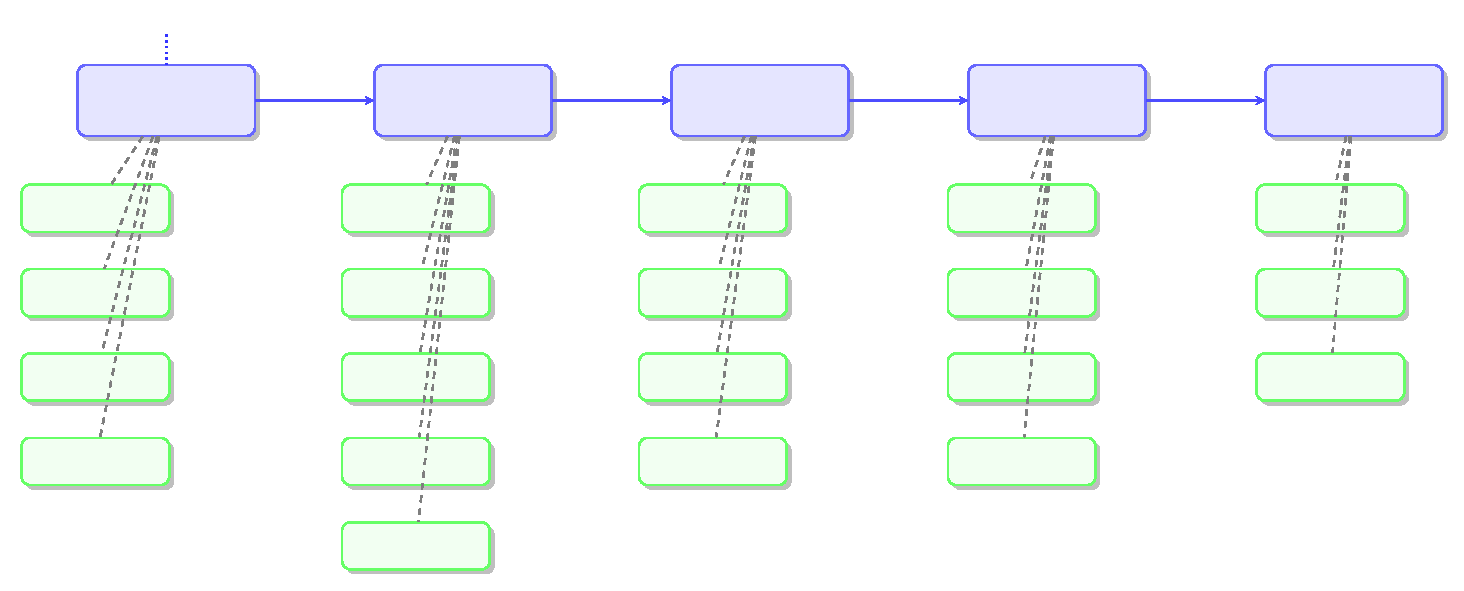
\includegraphics[width=0.95\textwidth]{figures/paper_structure.pdf}
% \caption{论文组织结构图}
% \label{fig:paper_structure}
% \end{figure}

% 更新历史:
% - 2026-03-20: 根据用户提供的参考图片，重新设计为横向流程图布局
%   * 使用TikZ绘制，包含标题框和五个章节框
%   * 第三章使用蓝色背景高亮，突出核心创新
%   * 使用箭头从标题指向各个章节，清晰展示结构关系
% - 2026-03-20 16:26: 参考学长论文风格，重新设计为简洁版
%   * 移除顶部的大标题框
%   * 简化文字描述，只保留核心要点
%   * 五个章节横向排列，用箭头连接表示逻辑关系
%   * 第三章仍用蓝色高亮突出
%   * 添加底部说明文字
%   * 字体更小，布局更紧凑
% - 2026-03-20 16:43: 突出2-5章的主线关系
%   * 第1章：绪论，作为引言部分单独呈现
%   * 第2-3-4章形成主线：背景→设计→实验
%   * 第3章为核心章节，用蓝色粗框+红色标记突出
%   * 第5章：总结展望，承接第4章
%   * 连接线标注逻辑关系：引入→支撑→验证→总结
% - 2026-03-20 17:07: 总分总上下结构
%   * 第1章在上方（总：引言）
%   * 第2-5章在下方横向排列（分+总）
%   * 第3章用蓝色粗框+红色标记突出核心
%   * 第5章用绿色框突出总结性质
%   * 从第1章向下连接到各章，表示从绪论展开
% - 2026-03-20 17:12: 中间分两边结构
%   * 第1章在上方（总：引言）
%   * 第2-4章在中间横向排列（分）：2左，3中，4右
%   * 第5章在下方（总：总结）
%   * 第3章用蓝色粗框+红色标记突出核心
%   * 连接线：1→2,3,4；2,3,4→5

% 设计理念:
% - 总分总上下结构：第1章在上方（总），第2-5章在下方（分+总）
% - 学长论文的布局：上1，下2345
% - 逻辑关系：绪论引入 → 背景支撑 → 系统设计 → 实验验证 → 总结展望

% =====================================================
% 图片2: 系统整体架构图
% 原始位置: fig:arch (chap03.tex, 第12行)
% 引用章节: 第三章 3.1节 系统整体架构
% 用途: 展示固件仿真系统的整体架构和模块关系
% =====================================================

% 原始TikZ代码:
% \begin{tikzpicture}[
%     module/.style={rectangle, draw=black!60, rounded corners=8pt, minimum width=4cm, minimum height=2cm, align=center, font=\small\bfseries, line width=1pt},
%     note/.style={font=\scriptsize, text=black!60, align=left},
%     arrow/.style={->, >=stealth, line width=1.5pt, draw=black!70}
% ]
%     \node[module, fill=orange!15] (static) at (-6, 0) {驱动函数接口\\静态分析与\\识别模块};
%     \node[note, below=0.3cm of static] {CodeQL分析\\MMIO识别\\函数定位\\数据模型};
%     \node[module, fill=green!15] (replace) at (0, 0) {驱动函数分析、\\替换与编译模块};
%     \node[note, below=0.3cm of replace] {LLM分类\\替换策略\\代码生成\\编译集成};
%     \node[module, fill=red!15] (feedback) at (6, 0) {动态测试\\反馈闭环模块};
%     \node[note, below=0.3cm of feedback] {仿真运行\\日志采集\\错误分析\\反馈回流};
%     \draw[arrow, draw=blue!60] (static.east) -- node[above, font=\scriptsize] {驱动函数列表} (replace.west);
%     \draw[arrow, draw=blue!60] (replace.east) -- node[above, font=\scriptsize] {替换代码} (feedback.west);
%     \draw[arrow, draw=red!60, dashed] (feedback.south) -- ++(0, -1) -- ++(-12, 0) -- ++(0, 0.8) node[midway, below, font=\scriptsize] {错误反馈} (replace.south);
% \end{tikzpicture}

% 更新说明:
% - 2026-03-20 20:40: 由于Poyo API无法连接，使用TikZ重新设计
%   * 现代简洁风格，三个主要模块横向排列
%   * 左侧：驱动函数接口静态分析与识别模块（橙色）
%   * 中间：驱动函数分析、替换与编译模块（蓝色，核心模块）
%   * 右侧：动态测试反馈闭环模块（绿色）
%   * 每个模块列出4个关键功能点
%   * 箭头连接：静态→核心→测试
%   * 红色虚线表示反馈闭环
%   * 添加阴影效果，视觉更美观
%   * 底部添加标题说明整体流程

% Poyo API问题:
% - 多次测试显示 api.poyo.app 连接超时
% - 无法使用Poyo生成图片
% - 使用TikZ作为替代方案，效果良好

% =====================================================
% 图片3: 动态执行与反馈多智能体架构图
% 原始位置: fig:multiagent-architecture (嵌入在chap03.tex中)
% 引用章节: 第三章 3.4节 (chap03.tex, 约790行)
% 用途: 展示动态测试反馈闭环的多智能体架构
% =====================================================

% 更新说明:
% - 2026-03-20 15:43: 重新设计为简洁的三排布局
% - 上排: Emulator Runner Agent (仿真运行)
% - 中排: Fixer Agent → Builder Agent (修复→构建)
% - 下排: 运行反馈 → 回归验证
% - 红色虚线箭头表示反馈闭环（回归→重新仿真）
% - 移除了所有工具节点的细节，只保留核心流程
% - 字体简化，减少文字描述

% 原始复杂版本特点:
% - 包含3个Agent + 1个MCP + 8个工具节点
% - 复杂的工具调用关系
% - 纵横交错的连接线
% - 用户反馈: 很乱的图

% 新版本特点:
% - 三排总分总布局，清晰简洁
% - 只展示核心Agent和主要流程
% - 闭环关系一目了然
% - 配色方案: 蓝色(仿真) → 橙色(修复) → 绿色(构建)


% =====================================================
% 图片1: 论文组织结构图
% 原始位置: figures/paper_structure.pdf
% 引用章节: 第一章 绪论 (chap01.tex, 第155行)
% 用途: 展示论文的整体组织结构和各章节内容
% =====================================================

% 原始引用代码:
% \begin{figure}[htbp]
% \centering
% 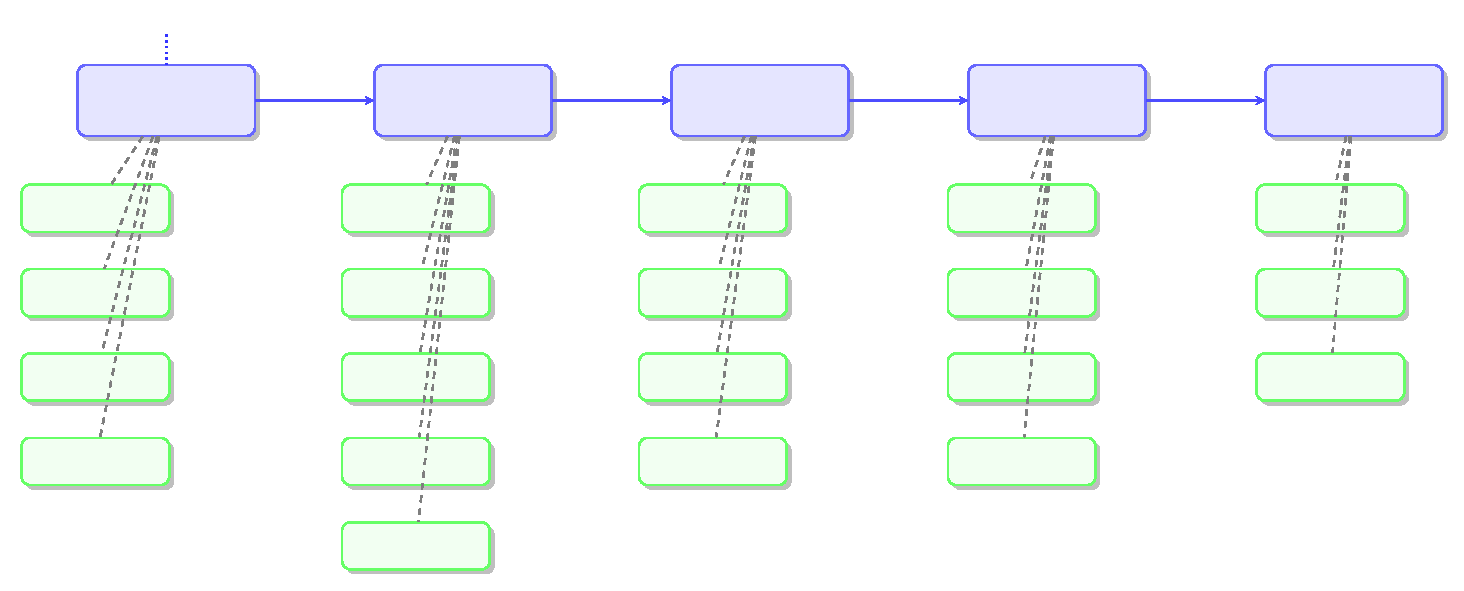
\includegraphics[width=0.95\textwidth]{figures/paper_structure.pdf}
% \caption{论文组织结构图}
% \label{fig:paper_structure}
% \end{figure}

% 更新历史:
% - 2026-03-20: 根据用户提供的参考图片，重新设计为横向流程图布局
%   * 使用TikZ绘制，包含标题框和五个章节框
%   * 第三章使用蓝色背景高亮，突出核心创新
%   * 使用箭头从标题指向各个章节，清晰展示结构关系
% - 2026-03-20 16:26: 参考学长论文风格，重新设计为简洁版
%   * 移除顶部的大标题框
%   * 简化文字描述，只保留核心要点
%   * 五个章节横向排列，用箭头连接表示逻辑关系
%   * 第三章仍用蓝色高亮突出
%   * 添加底部说明文字
%   * 字体更小，布局更紧凑
% - 2026-03-20 16:43: 突出2-5章的主线关系
%   * 第1章：绪论，作为引言部分单独呈现
%   * 第2-3-4章形成主线：背景→设计→实验
%   * 第3章为核心章节，用蓝色粗框+红色标记突出
%   * 第5章：总结展望，承接第4章
%   * 连接线标注逻辑关系：引入→支撑→验证→总结
% - 2026-03-20 17:07: 总分总上下结构
%   * 第1章在上方（总：引言）
%   * 第2-5章在下方横向排列（分+总）
%   * 第3章用蓝色粗框+红色标记突出核心
%   * 第5章用绿色框突出总结性质
%   * 从第1章向下连接到各章，表示从绪论展开
% - 2026-03-20 17:12: 中间分两边结构
%   * 第1章在上方（总：引言）
%   * 第2-4章在中间横向排列（分）：2左，3中，4右
%   * 第5章在下方（总：总结）
%   * 第3章用蓝色粗框+红色标记突出核心
%   * 连接线：1→2,3,4；2,3,4→5

% 设计理念:
% - 中间分两边结构：上1，中2-3-4，下5
% - 第1章绪论引出，第2-4章展开，第5章总结
% - 第3章核心章节在正中间，突出显示
% - 布局对称美观，逻辑清晰

% =====================================================
% 图片2: 动态执行与反馈多智能体架构图
% 原始位置: fig:multiagent-architecture (嵌入在chap03.tex中)
% 引用章节: 第三章 3.4节 (chap03.tex, 约790行)
% 用途: 展示动态测试反馈闭环的多智能体架构
% =====================================================

% 更新说明:
% - 2026-03-20 15:43: 重新设计为简洁的三排布局
% - 上排: Emulator Runner Agent (仿真运行)
% - 中排: Fixer Agent → Builder Agent (修复→构建)
% - 下排: 运行反馈 → 回归验证
% - 红色虚线箭头表示反馈闭环（回归→重新仿真）
% - 移除了所有工具节点的细节，只保留核心流程
% - 字体简化，减少文字描述

% 原始复杂版本特点:
% - 包含3个Agent + 1个MCP + 8个工具节点
% - 复杂的工具调用关系
% - 纵横交错的连接线
% - 用户反馈: 很乱的图

% 新版本特点:
% - 三排总分总布局，清晰简洁
% - 只展示核心Agent和主要流程
% - 闭环关系一目了然
% - 配色方案: 蓝色(仿真) → 橙色(修复) → 绿色(构建)
